\documentclass[a4paper, 11pt]{article}
\usepackage[utf8]{inputenc} 
\usepackage[T1]{fontenc}
%\usepackage{lmodern}
\usepackage{graphicx}
\usepackage[english]{babel}
\usepackage[left=2cm,right=2cm,top=1.5cm,bottom=2cm]{geometry}
\usepackage{fancyhdr}
\usepackage{amsmath,amsfonts,amssymb}
\usepackage{lastpage}
\usepackage{times}
%\usepackage[dvips]{graphicx}
\usepackage{epsfig}
\usepackage{amsmath}
%\usepackage{pgf,pgfarrows,pgfautomata,pgfheaps,pgfnodes,pgfshade}
\usepackage[useregional]{datetime2}
%\usepackage[amsmath]{maxiplot}

\usepackage{xcolor, soul}
%\sethlcolor{green}

\usepackage{tikz,tkz-tab}
\usepackage{tabularx}

\usepackage{moreverb}
\usepackage{hyperref}

\usepackage{makeidx} 
\makeindex

\usepackage{multicol}
\usepackage[tikz]{bclogo}
\usepackage{array}

\usepackage[shortlabels]{enumitem}
%\setlist[itemize,1]{label=$\star$}
\setlist[itemize,1]{label=\textbullet}
\setlist[itemize,2]{label=$\diamondsuit$} 

\renewcommand{\headrulewidth}{0.0pt}
\renewcommand{\footrulewidth}{0.5pt}

\setlength{\parindent}{0pt}

\newcounter{num}
\renewcommand{\thenum}{\Roman{num}}
\newcommand{\exo}{\addtocounter{num}{1}{\noindent \textbf{Exercise~\thenum~:}}}
\newenvironment{exercice}{\exo}{\vspace{0.4cm}}
\newcommand{\version}{2.0}

\begin{document}

\pagestyle{fancy} \lhead{} \chead{} \rhead{} 
\rfoot{\small{{\thepage/\pageref{LastPage}}}} 
\cfoot{Version \version} 
\lfoot{mac2texpdf2 Software}

\setcounter{tocdepth}{2}
\renewcommand*{\contentsname}{Table of Contents}

\fbox{\makebox[\textwidth][c]{\textbf{
\LARGE mac2texpdf2 Software Documentation
}}}

\begin{center}
{\large \textbf{Version \version{} dated \today} \\
Author: Michel Gosse, michel.gosse@free.fr}
\end{center}

 
%\tableofcontents

\section*{Overview}
This software is a utility that allows you to enter commands for the Maxima software (either by typing them or after a copy/paste) which generates a PDF file containing the entered commands as well as the results calculated by Maxima. It also allows the export of the \LaTeX{} file used to produce the PDF as well as the document images to a folder chosen by the user.

\subsection*{Screenshots}

\begin{figure}[ht]
  \centering
  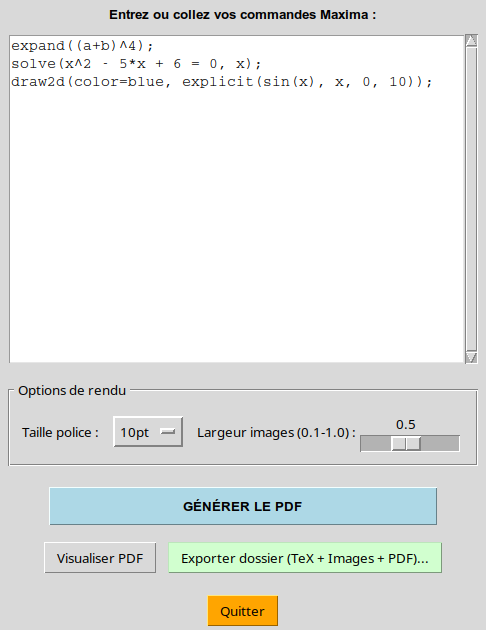
\includegraphics[width=0.45\textwidth]{img1mac2tex.png}% 
  \hspace{0.05\textwidth}%
  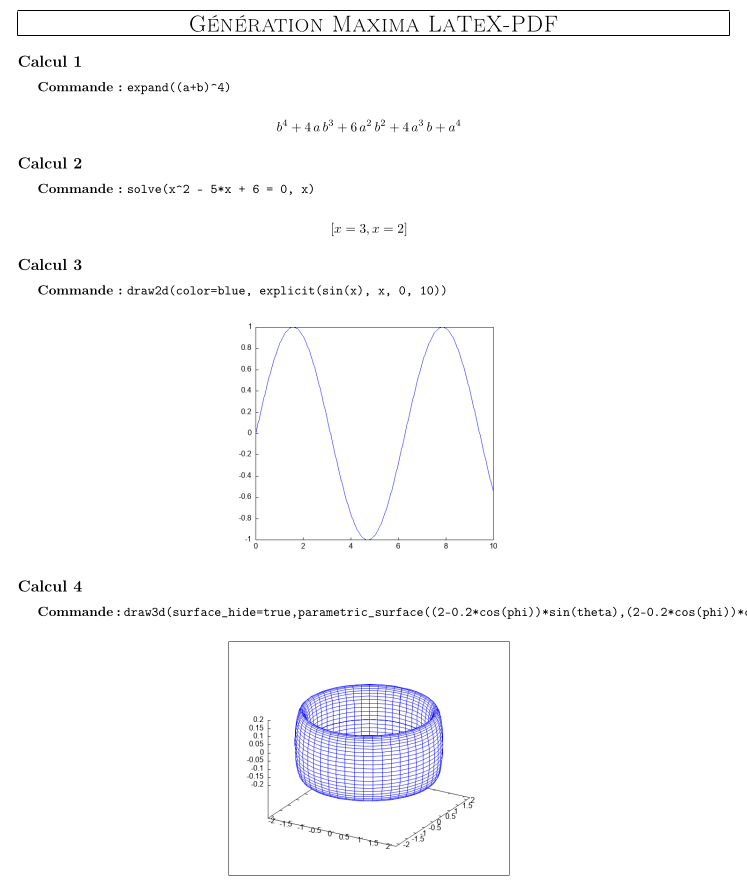
\includegraphics[width=0.45\textwidth]{img3mac2tex.png}
\end{figure}

\subsection*{Software Principle}

The software sends commands to the Maxima computer algebra system (line by line), which executes them and returns the result in \LaTeX{}. The software retrieves this data and formats it in a \LaTeX{} document which is then compiled with pdflatex. It is a Python script, which is also available as an executable for Windows or Linux.

\subsection*{Comparison with wxMaxima}

This utility is a lightweight and fast tool that allows you to quickly obtain a high-quality document containing the results calculated by Maxima from commands entered by the user (in PDF or \LaTeX{} format). It does not offer the power of wxMaxima and is not suitable for solving complex exercises.

\subsection*{Prerequisites}

To function, the software requires:
\begin{enumerate}
\item Maxima software
\item Gnuplot software 
\item A \LaTeX{} distribution including the following packages: xcolor, listings, datetime2, babel, geometry, fancyhdr, lastpage, graphicx, mathtools, amsmath, amsfonts, asmssymb
\item If you wish to use the source version (the Python script), then Python must also be installed on the computer.
\end{enumerate} 

\emph{The various installations are detailed by operating system below.}

\section*{Installation for Windows}

\subsection*{Step 1: Install Maxima and add Maxima to the PATH}
$\blacktriangleright$ Download and install Maxima (version 5.49.0):
\begin{center}
\href{https://sourceforge.net/projects/maxima/files/Maxima-Windows/5.49.0-Windows/}
{https://sourceforge.net/projects/maxima/files/Maxima-Windows/5.49.0-Windows/}
\end{center}

$\blacktriangleright$ Modify environment variables:
\begin{enumerate}
\item Open settings: Windows Key + I
\item Go to System → About.
\item Click on Advanced system settings.
\item In the window that opens, click on the Environment Variables… button at the bottom
\item Choose PATH and modify
\item Add the two lines at the end of the text \\
C:\textbackslash maxima-5.49.01 \textbackslash bin \\
C:\textbackslash maxima-5.49.01 \textbackslash gnuplot \textbackslash bin
\item Validate with OK several times to close all windows
\end{enumerate}

\textit{Note}: Gnuplot software is automatically installed at the same time as Maxima.

\subsection*{Step 2: Installation of a \LaTeX{} distribution}
If \LaTeX{} is installed, verify that the packages xcolor, listings, datetime2, babel, geometry, fancyhdr, lastpage, graphicx, mathtools, amsmath, amsfonts, asmssymb are properly installed.

Otherwise, download the Texlive distribution and install it (it automatically installs all required packages and modifies the PATH directly):

\begin{center}
\href{https://tug.org/texlive/windows.html}{https://tug.org/texlive/windows.html}
\end{center}

\subsection*{Step 3 (optional): Python installation}

If you wish to use the Python script and not the executable, you must install Python (the installation also adds it to the PATH automatically).

\begin{center}
\href{https://www.python.org/downloads/windows/}{https://www.python.org/downloads/windows/}
\end{center}

\subsection*{Step 4: Download the mac2texpdf2-eng.exe software}
Download the Windows version from the page:

\begin{center}
\href{https://maxima-french-doc.fr/interfaces/}{https://maxima-french-doc.fr/interfaces/}
\end{center}
You just need to unzip the file and double-click on the Windows executable retrieved (it is called mac2texpdf2-eng-w.exe).

Windows issues a warning indicating that the software is not certified. To launch it, you must accept to run unknown software...

\textbf{Alternative with Python: download the Python script mac2texpdf2-eng-w.py}

Once unzipped, you need to open a command prompt, navigate to the folder containing the Python file, and type the command:
\textit{python mac2texpdf2-eng--w.py}

\section*{Installation for Linux}

\subsection*{Step 1: Install Maxima}
If the software is not installed, you can either install it via your distribution's package manager, or download it from the page:

\begin{center}
\href{https://sourceforge.net/projects/maxima/files/Maxima-Linux/5.49.0-Linux/}{https://sourceforge.net/projects/maxima/files/Maxima-Linux/5.49.0-Linux/}
\end{center}
The PATH is added automatically (unlike Windows).

\subsection*{Step 2: Install \LaTeX{}}
To be done with your distribution's package manager. A complete installation should be performed to have all required packages. Otherwise, they are contained in the texlive-latex-extra package.

\subsection*{Step 3 (optional): Python installation}
If you wish to use the Python script and not the binary, install Python via your distribution's package manager.

\subsection*{Step 4: Download the mac2texpdf2-eng.bin software}
Download the Linux version from the page:

\begin{center}
\href{https://maxima-french-doc.fr/interfaces/}{https://maxima-french-doc.fr/interfaces/}
\end{center}
You just need to unzip the file and double-click on the Linux binary retrieved (it is called mac2texpdf2-eng.bin).

\textbf{Alternative with Python: download the Python script mac2texpdf2-eng.py}

Once unzipped, you need to open a terminal, navigate to the folder containing the Python file, and type the command:
\textit{python3 mac2texpdf2-eng.py}


\section*{Using mac2texpdf2}

The operation is very simple:
\begin{itemize}
\item Enter a series of Maxima commands in the text area. \emph{Each command is on a single line and must end with a ;}
\item Choose the font size for the PDF that will be generated. If there are graphics, choose the scale for the graphics (between 0 and 1).
\item Click on Generate PDF
\item Click on View PDF. 
\item If you want to retrieve the PDF and the corresponding \LaTeX{} file (with the document images), click on the export folder button.
\end{itemize}

\subsection*{Some points of attention}

\begin{itemize}
\item For graphics, use the draw2d and draw3d commands. The wxdraw2d and wsdraw3d commands are specific to wxMaxima software and are not recognized by Maxima which ignores them.
\item Since Maxima input/output is not numbered by mac2texpdf2 software, you cannot use \% to designate the previous result.
For example:
\begin{verbatim}
solve(a*x^2-1=0,x);
subst(5,a,%);
\end{verbatim}
does not work. Instead, each result must be named to be used later:
\begin{verbatim}
eq:solve(a*x^2-1=0,x);
subst(5,a,eq);
\end{verbatim}
\end{itemize}

\section*{Links and references}

\subsection*{Maxima documentation}
\href{https://maxima-french-doc.fr/documentation/}{https://maxima-french-doc.fr/documentation/}

\subsection*{mac2texpdf2 software page}
\href{https://maxima-french-doc.fr/interfaces/}{https://maxima-french-doc.fr/interfaces/}

\subsection*{mac2texpdf2 software development site}
The software is under development in a GitHub repository:

\href{https://github.com/michelprog59/mac2texpdf2}{https://github.com/michelprog59/mac2texpdf2}

\subsection*{License and contact}
The software is distributed under the GNU GENERAL PUBLIC LICENSE (GPL) v3.0 and can be used and modified freely.

For any development requests or bug reports, you can either do so directly on GitHub, or send me an email at michel.gosse@free.fr

\end{document}
